Diferente da figura \ref{module}, o foco da figura \ref{classdiagrama} consiste em apresentar como se da a estrutura de classes e dos relacionamentos. 
Ambas situações poderiam ser representadas em uma única figura, contudo os pesquisadores decidiram por seccionar em duas a fim de tornar o processo 
mais didatico. Por esse mesmo motivo não está apresentado neste \textit{UML} todas as classes e propriedades.  

\begin{figure}[H]
  \centering
  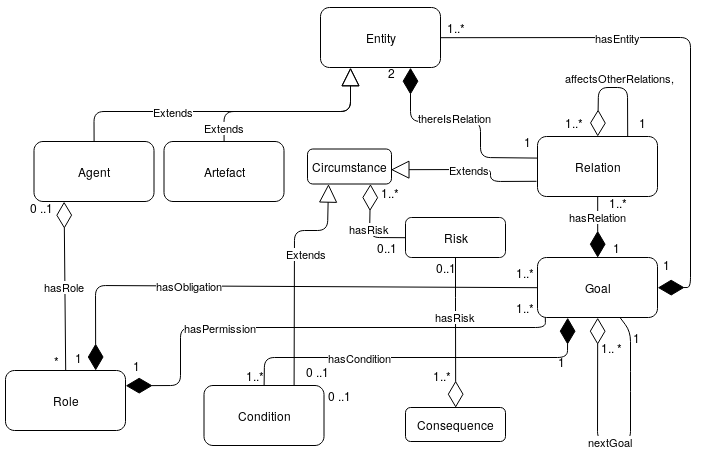
\includegraphics[width=1\linewidth]{figure/Class.png} 
  \caption{Diagrama de classes do Modelo }
  \label{classdiagrama}
\end{figure}

Uma vantagem deste tipo de diagrama em relação a representação por conjuntos consiste na ocorrência de uma semântica específica para tratar dois pontos
relevantes dentro do contexto computacional: cardinalidade e relações existenciais. Um dos predicados interessantes de serem analisados, neste contexto, 
é \textit{hasRole} que define um relacionamento fracamente agregado entre \textit{Agent} e \textit{Role}. Isso, pois (dentro do escopo deste modelo) um 
agente pode existir sem ter um papel, portanto este não é um critério necessário para definir aquele. A cardinalidade se justifica tendo como base o fato 
de que um agente pode ter um ou mais papeis. 

As relações \textit{hasObligation}, \textit{hasPermission} se dão por meio de agregações fortes tendo vista que não há sentido semântico para um papel 
$\rho$ existir sem que esteja vinculado a ao menos um objetivo. Como um papel se relaciona com diversos objetivos, os engenheiros adotaram a cardinalidade 
de $1$ para $1 .. *$.

A relação \textit{hasRisk} ocorre entre $Consequence$,$Condition$, $Relation$ e $Risk$. Contudo, uma esse relacionamento 
não se dá entre as quatro classes no mesmo instante, sendo assim: $Consequence$,$Condition$,$Risk$ ou assim:$Consequence$,$Relation$,$Risk$. A representação 
desta situação presente na subseção \ref{predic} se deu de forma relativamente simples, criando uma variável que poderia assumir instâncias de $Relation$ 
ou de $Condition$. Contudo, isso não se aplica em UML. Para resolver esse problema, os engenheiros criaram uma classe chamada $Circumstance$, que é pai 
de $Relation$ e de $Condition$. Essa classe não possui sentido semântico dentro do modelo e sua existência se deve apenas para resolver esse problema 
neste tipo de linguagem de representação. De 0 a 1 risco pode ter 1 ou mais relacionamentos com $Circumstance$ e o mesmo ocorre com $Consequence$. 

Um objetivo não pode ser definido sem saber quais são as entidades $Entity$, relações $Relation$ e consequências $Consequence$ necessários para que 
seja alcançado. Por isso os predicados $hasCondition$,$hasEntity$ e $hasRelation$ estabelecem composição forte de suas respectivas classes com $Goal$. 
Como um objetivo pode apontar para diversas instancias dessas classes, os pesquisadores optaram - para cada uma das relações - trabalhar com a cardinalidade 
$1 - 1 .. *$.

No modelo roda relaçao $Relation$ deve estar relacionada com duas entidades. Por esse motivo o predicado $thereIsRelation$ faz composição forte com 
$Entity$ e a sua cardinalidade é dada $1 - 2$. 

A classe $Goal$ possui uma relação consigo mesma dada por $nextGoal$. Essa é uma agregação fraca, pois do contrários seria impossível haver uma única instância desta classe. 
Isso se deve ao fato de que a primeira instância necessitaria de uma instância de $Goal$ para existir. Contudo, como não há um elemento de $Goal$ antes 
do primeiro elemento de $Goal$, logo esse primeiro elemento não pode existir. Um objetivo poder ter como próximo um ou mais objetivos, justificando 
a ocorrência da cardinalidade $1 .. n$. 

O predicao $affectsOtherRelations$, por motivos similares a $nextGoal$ deve ter agregação fraca. Como uma relação pode afetar uma ou mais, a cardinalidade 
adequada para essa circunstância é dada pro $1$ - $1 ..*$